% Toolbar icon: edit / rename — a pencil pointing to the lower-left (writing tip)
% with a body and a nib, in the shared monochrome line style.
\documentclass[tikz,border=2mm]{standalone}
\usetikzlibrary{arrows.meta,calc,shapes.geometric}
\begin{document}
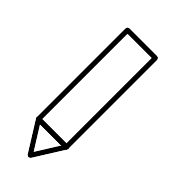
\begin{tikzpicture}[line width=1.8pt, line cap=round, line join=round, >=Stealth, x=1mm,y=1mm]
  % Pencil body (a rectangle along the 45° axis).
  \draw (-6.94,-3.4) -- (4.37,7.9) -- (7.9,4.37) -- (-3.4,-6.94) -- cycle;
  % Nib: the triangular tip at the writing end.
  \draw (-6.94,-3.4) -- (-8,-8) -- (-3.4,-6.94);
  % Collar line between wood and lead.
  \draw (-6.94,-3.4) -- (-3.4,-6.94);
\end{tikzpicture}
\end{document}
